% ---
% Classe para documento digital (não impresso) - formato oneside
% ---
\documentclass[
  12pt,
  oneside,
  a4paper,
  english,
  brazilian
  ]{abntex2}

% ---
% Pacotes básicos
% ---
\usepackage[scaled]{helvet}
\renewcommand{\familydefault}{\sfdefault}
\usepackage[T1]{fontenc}
\usepackage[utf8]{inputenc}
\usepackage{indentfirst}
\usepackage{color}
\usepackage{graphicx}
\usepackage{microtype}
\usepackage{lipsum}

\setlength{\marginparwidth}{2cm}
\usepackage[portuguese]{todonotes}
\usepackage{tikz}
\usetikzlibrary{arrows.meta, positioning}   % bibliotecas extras para grafos dirigidos
\usepackage{amsmath, amssymb}

% ---
% Pacotes de citações
% ---
\usepackage[alf]{abntex2cite}

% ---
% Ajustes de fonte para títulos
% ---
\renewcommand{\ABNTEXchapterfont}{\sffamily\bfseries}
\renewcommand{\ABNTEXchapterfontsize}{\LARGE}
\renewcommand{\ABNTEXsectionfont}{\sffamily\bfseries}
\renewcommand{\ABNTEXsectionfontsize}{\Large}
\renewcommand{\ABNTEXsubsectionfont}{\sffamily\bfseries}
\renewcommand{\ABNTEXsubsectionfontsize}{\large}

\renewcommand{\thepage}{\arabic{page}}
\renewcommand{\thechapter}{\arabic{chapter}}
\renewcommand{\thesection}{\thechapter.\arabic{section}}
\renewcommand{\thesubsection}{\thesection.\arabic{subsection}}
\renewcommand{\thefigure}{\arabic{figure}}
\renewcommand{\thetable}{\arabic{table}}

\captionstyle{\sffamily\bfseries}
\captionnamefont{\sffamily\bfseries}
\captiontitlefont{\sffamily}

% ---
% Proteção para Metadados do PDF
% ---
\pdfstringdefDisableCommands{%
  \def\\{ }%
  \def\par{ }%
  \def\vspace#1{ }%
  \def\sffamily{}%
  \def\bfseries{}%
}

% ---
% Arquivo de Bibliografia Embutido
% ---
\begin{filecontents*}{referencias.bib}

@misc{fabricio2019,
  author = {Siqueira, Fabrício and others},
  title  = {Portal OBMEP: Material Teórico -- Tópicos Adicionais --
            Introdução à Teoria Dos Grafos -- Parte 1},
  year   = {2019}
}

@book{boaventura2009,
  author    = {Boaventura, Oswaldo and Jurkiewicz, Samuel},
  title     = {Grafos},
  publisher = {Editora Blucher},
  year      = {2009}
}

@misc{silva2020,
  author = {Da Silva, Luiz Fernando},
  title  = {Uma Proposta de Sequência Didática para o Ensino Médio:
            Introdução ao Estudo da Teoria dos Grafos com GeoGebra},
  year   = {2020},
  note   = {6 mai. 2020}
}

@book{cormen2009,
  author    = {Cormen, T. H. and Leiserson, C. E. and Rivest, R. L. and Stein, C.},
  title     = {Introduction to Algorithms},
  edition   = {3},
  publisher = {MIT Press},
  address   = {Cambridge, Mass.},
  year      = {2009}
}

@mastersthesis{custodio2025,
  author  = {Custodio, Diego Scanavachi},
  title   = {Um estudo sobre grafos e sua aplicabilidade no ensino médio},
  school  = {Universidade de São Paulo},
  address = {São Carlos},
  year    = {2025},
  note    = {Disponível em:
             \url{https://www.teses.usp.br/teses/disponiveis/55/55136/tde-24072025-110655/}.
             Acesso em: 4 nov. 2025}
}

@manual{brasil2002,
  organization = {Brasil},
  title        = {{PCN+} Ensino Médio: Orientações Educacionais Complementares
                  aos Parâmetros Curriculares Nacionais -- Ciências da Natureza,
                  Matemática e suas Tecnologias},
  address      = {Brasília},
  publisher    = {MEC/SEMTEC},
  year         = {2002}
}

@misc{figueredo,
  author = {Figueredo, J.},
  title  = {Teoria dos Grafos: Representação de Grafos}
}

@misc{jurkiewicz2007,
  author = {Jurkiewicz, S.},
  title  = {Grafos: Uma introdução},
  year   = {2007},
  note   = {Programa de Iniciação Científica da OBMEP 2007}
}

@book{lopes2010,
  author    = {Lopes, M. L. M. L.},
  title     = {Grafos: jogos e desafios},
  address   = {Rio de Janeiro},
  publisher = {IM/UFRJ},
  year      = {2010}
}

@mastersthesis{malta2008,
  author  = {Malta, G. H. S.},
  title   = {Grafos no ensino médio: uma inserção possível},
  school  = {Universidade Federal do Rio Grande do Sul},
  address = {Porto Alegre},
  year    = {2008}
}

@book{santos2007,
  author    = {Santos, J. P. O. and Mello, M. P. and Murari, I. T. C.},
  title     = {Introdução à Análise Combinatória},
  edition   = {4},
  address   = {Rio de Janeiro},
  publisher = {Editora Ciência Moderna},
  year      = {2007}
}

@article{rodrigues2021,
  author  = {Rodrigues, A. B. and Silva, C. D.},
  title   = {O ensino de grafos e a cultura digital: novas perspectivas
             para a matemática escolar},
  journal = {Revista de Educação Matemática},
  volume  = {10},
  number  = {2},
  pages   = {1--15},
  year    = {2021}
}

% ---------------------------------------------------------------
% Referências adicionadas para sustentar as definições e exemplos
% ---------------------------------------------------------------

@book{diestel2017,
  author    = {Diestel, Reinhard},
  title     = {Graph Theory},
  edition   = {5},
  publisher = {Springer},
  address   = {Berlin},
  year      = {2017}
}

@book{wilson1996,
  author    = {Wilson, Robin J.},
  title     = {Introduction to Graph Theory},
  edition   = {4},
  publisher = {Longman},
  address   = {London},
  year      = {1996}
}

@book{bondy1976,
  author    = {Bondy, J. A. and Murty, U. S. R.},
  title     = {Graph Theory with Applications},
  publisher = {North-Holland},
  address   = {New York},
  year      = {1976}
}

@book{rosen2012,
  author    = {Rosen, Kenneth H.},
  title     = {Discrete Mathematics and Its Applications},
  edition   = {7},
  publisher = {McGraw-Hill},
  address   = {New York},
  year      = {2012}
}

@article{euler1736,
  author  = {Euler, Leonhard},
  title   = {Solutio problematis ad geometriam situs pertinentis},
  journal = {Commentarii Academiae Scientiarum Imperialis Petropolitanae},
  volume  = {8},
  pages   = {128--140},
  year    = {1741},
  note    = {Apresentado em 1736}
}

@misc{brasil1996,
  author   = {Brasil},
  title    = {Lei n\textordmasculine{} 9.394, de 20 de dezembro de 1996:
              Estabelece as diretrizes e bases da educação nacional},
  address  = {Brasília},
  year     = {1996},
  note     = {Diário Oficial da União, Brasília, DF, 23 dez. 1996.
              Disponível em: \url{http://www.planalto.gov.br/ccivil_03/leis/l9394.htm}.
              Acesso em: 10 jan. 2026}
}

\end{filecontents*}

% ---
% Informações de dados para CAPA e FOLHA DE ROSTO
% ---
\titulo{PROPOSTA DE INSERÇÃO DO ENSINO DE GRAFOS: PARA ALUNOS DO ENSINO MÉDIO DA REDE PÚBLICA DE ENSINO}
\autor{JOSÉ GUILHERME DANTAS SILVA}
\local{Ilhéus-BA}
\data{2026}
\orientador{Prof. Dr. Romenique da Rocha Silva}
\coorientador[Coorientadora:]{Prof\textsuperscript{a}. Ma. Sara Meira Moutta}
\instituicao{%
  UNIVERSIDADE ESTADUAL DE SANTA CRUZ
  \par
  Departamento de Ciências Exatas
  \par
  Licenciatura em Matemática}
\tipotrabalho{Trabalho de Conclusão de Curso}
\preambulo{Trabalho de Conclusão de Curso apresentado ao curso de Licenciatura em Matemática, Departamento de Ciências Exatas, da UNIVERSIDADE ESTADUAL DE SANTA CRUZ, como requisito parcial para a obtenção do grau de Licenciado em Matemática.}

% ---
% Redefinição da Capa
% ---
% ---
% Capa padrão ABNT NBR 14724:2011
% Estrutura: Instituição (topo) → Autor (fixo, próximo ao topo) →
%            Título (centro) → Local / Ano (rodapé)
% ---
\renewcommand{\imprimircapa}{%
  \begin{capa}%
    \centering
    % ---- Cabeçalho: brasão + nome da instituição ----
    
\includegraphics[width=3cm]{Brasão-UESC---png1.png}\\[0.4cm]
    {\ABNTEXchapterfont\large\imprimirinstituicao}

    \vspace{2.5cm} % espaço fixo — autor fica no terço superior

    % ---- Autor ----
    {\ABNTEXchapterfont\large\imprimirautor}

    \vspace*{\fill} % espaço elástico empurra o título para o centro

    % ---- Título ----
    {\ABNTEXchapterfont\bfseries\LARGE\imprimirtitulo}

    \vspace*{\fill} % espaço elástico empurra local/ano para o rodapé

    % ---- Local e Ano ----
    {\large\imprimirlocal}\\[0.3cm]
    {\large\imprimirdata}\\[1cm]
  \end{capa}
}

% ---
% Configurações de aparência do PDF final
% ---
\definecolor{blue}{RGB}{41,5,195}

\hypersetup{
    pdftitle  = {\imprimirtitulo},
    pdfauthor = {\imprimirautor},
    colorlinks = true,
    linkcolor  = blue,
    citecolor  = blue,
    urlcolor   = blue
}

\setlength{\parindent}{1.3cm}
\setlength{\parskip}{0.2cm}

% ============================================================
% INÍCIO DO DOCUMENTO
% ============================================================
\begin{document}
\selectlanguage{brazilian}
\frenchspacing

% ----------------------------------------------------------
% ELEMENTOS PRÉ-TEXTUAIS
% ----------------------------------------------------------
\pretextual

\imprimircapa
\imprimirfolhaderosto*

% ---
% Folha de aprovação
% ---
\begin{folhadeaprovacao}
  \begin{center}
    {\ABNTEXchapterfont\large\imprimirautor}
    \vspace*{\fill}\vspace*{\fill}
    \begin{center}
      \ABNTEXchapterfont\bfseries\Large\imprimirtitulo
    \end{center}
    \vspace*{\fill}
    \hspace{.45\textwidth}
    \begin{minipage}{.5\textwidth}
        \imprimirpreambulo
    \end{minipage}%
    \vspace*{\fill}
  \end{center}

  Aprovado em: Ilhéus, \_\_ de \_\_\_\_\_\_\_\_\_\_\_\_ de \_\_\_\_.

  \begin{center}
    \vspace*{0.5cm}
    \textbf{BANCA EXAMINADORA} \\
    \vspace*{1.5cm}
    \hrulefill \\
    \textbf{\imprimirorientador} (Orientador) \\
    Universidade Estadual de Santa Cruz \\
    \vspace*{1.5cm}
    \hrulefill \\
    \textbf{\imprimircoorientador} (Coorientadora) \\
    Universidade Estadual de Santa Cruz \\
    \vspace*{1.5cm}
    \hrulefill \\
    \textbf{Prof\textsuperscript{a}. Dr\textsuperscript{a}.\ Jurema Lindote Botelho Peixoto} (Examinadora) \\
    Universidade Estadual de Santa Cruz \\
  \end{center}
\end{folhadeaprovacao}

% ---
% Dedicatória
% ---
\begin{dedicatoria}
   \vspace*{\fill}
   \centering
   \noindent
   \textit{Dedico este trabalho in memoriam a meu pai, Geraldo Bezerra da Silva,
           como homenagem à sua vida e legado.}
   \vspace*{\fill}
\end{dedicatoria}

% ---
% Agradecimentos
% ---
\begin{agradecimentos}
Gostaria de começar agradecendo a Deus, que, com sua infinita bondade e
misericórdia, me deu forças e me capacitou para chegar até aqui. Sei, inclusive,
que Ele ainda me fará ir muito mais longe.

Agradeço à Universidade Estadual de Santa Cruz (UESC), instituição de excelência
que me proporcionou anos de grande enriquecimento, tanto intelectual quanto
espiritual. Tenho certeza de que retornarei a esta casa para cursar uma
pós-graduação e, futuramente, contribuir como docente.

Registro minha gratidão, de forma especial, ao meu orientador, professor
Dr.\ Romenique da Rocha Silva, cuja linha de pesquisa, especialmente no doutorado,
despertou em mim ainda mais fascínio pela área de computação e grafos. Esse
encantamento motivou a realização deste trabalho, com o qual pretendo contribuir
para a educação básica. Agradeço por sua presença constante, dedicação e empenho
em ler esta monografia com atenção, tornando-a uma pesquisa de excelência. Sou
igualmente grato pela amizade que cultivamos ao longo desse tempo e sei que ainda
estaremos juntos em outros projetos.

Expresso também meus agradecimentos a duas instituições da educação básica: o
Colégio Municipal Antônio Lima de Oliveira e o Colégio Estadual do Salobrinho.
Obrigado por acreditarem em mim, mesmo antes da hora, e por me permitirem
realizar o sonho de ser professor. A todos os alunos que passaram por mim, deixo
o reconhecimento: vocês foram fundamentais para que eu continuasse. Em muitos
momentos, pensei em desistir, mas vocês me mostraram a beleza da docência e me
deram forças para seguir.

Sou profundamente grato às pessoas que tornaram este sonho possível. À minha mãe,
Edileusa Gualberto Dantas (Inha), à minha avó, Doraci Maria da Silva (Vó Peró),
e às minhas irmãs, Victória Regina (Vick) e Claudineia (Lela), que nunca
deixaram de acreditar em mim, mesmo quando eu duvidava de mim mesmo.

Ao meu gato Bimbo, que esteve comigo em meio a noites em claro, compartilhando
angústias, com fórmulas espalhadas em papéis na garagem.

Ao meu colega e amigo Juan Cerqueira (Calopsita), meu parceiro de graduação que
se tornou um irmão: sem o seu apoio, companheirismo e cumplicidade, eu não teria
resistido. Sou imensamente grato por sua vida e sei que ainda vamos brilhar muito
juntos.

Por fim, agradeço aos meus supervisores de estágio e PIBID, Prof.\ Wellingthon
Fraga, Prof\textsuperscript{a}.\ Luana Cerqueira e Prof\textsuperscript{a}.\
Daniella Feitosa. Só tenho a agradecer a vocês por todo o ensinamento docente e
pela oportunidade de vivenciar experiências em sala de aula. Não poderia deixar
de mencionar também meu professor do ensino médio, Ms.\ Edmilson Chaves, que
despertou em mim, ainda na educação básica, o desejo de me tornar docente, e a
professora Dr\textsuperscript{a}.\ Jurema Peixoto, que acreditou em mim desde o
início da graduação.
\end{agradecimentos}

% ---
% Epígrafe
% ---
\begin{epigrafe}
    \vspace*{\fill}
  \begin{flushright}
    \textit{``A vida é como a matemática, criamos raízes \\
    que o mundo tenta subtrair de nós, porém o que é somado \\
    de bom nos ajudará a ter a solução exata do que precisamos.''\\
    (Ester Menezes)}
  \end{flushright}
\end{epigrafe}

% ---
% Resumos
% ---
\begin{resumo}
 [Insira aqui o texto do seu resumo de 150 a 500 palavras]
 \vspace{\onelineskip}
 \noindent
 \textbf{Palavras-chave}: Teoria dos Grafos. Ensino Médio. Matemática. BNCC.
\end{resumo}

\begin{resumo}[Abstract]
 \begin{otherlanguage*}{english}
   [Insert the abstract text here]
   \vspace{\onelineskip}
   \noindent
   \textbf{Keywords}: Graph Theory. High School. Mathematics. BNCC.
 \end{otherlanguage*}
\end{resumo}

\pdfbookmark[0]{\listfigurename}{lof}
\listoffigures*
\cleardoublepage

\begin{siglas}
  \item[BNCC] Base Nacional Comum Curricular
  \item[LDB]  Lei de Diretrizes e Bases da Educação Nacional
  \item[UESC] Universidade Estadual de Santa Cruz
\end{siglas}

\pdfbookmark[0]{\contentsname}{toc}
\tableofcontents*
\cleardoublepage

% ----------------------------------------------------------
% ELEMENTOS TEXTUAIS
% ----------------------------------------------------------
\textual

% ==========================================================
\chapter{INTRODUÇÃO}
% ==========================================================

A contextualização do ensino da Matemática na Educação Básica, particularmente
no Ensino Médio, demanda uma constante atualização curricular que dialogue com a
complexidade e a interconectividade do mundo contemporâneo. Nesse cenário, a
Teoria dos Grafos destaca-se não apenas como um ramo fundamental da Matemática
Discreta, mas como uma ferramenta indispensável para a modelagem e a compreensão
de fenômenos reais.

A relevância desse campo transcende a abstração teórica, manifestando-se
diretamente em estruturas que definem a sociedade atual, tais como a arquitetura
de redes sociais, o planejamento eficiente de sistemas de transporte e logística,
o funcionamento de algoritmos de busca e a análise de grandes volumes de dados
(\textit{Big Data}). Compreender grafos é, portanto, compreender a linguagem
estrutural por trás dos problemas de otimização e conectividade que permeiam o
cotidiano.

Para além de sua onipresença tecnológica, o estudo de grafos apresenta uma vasta
aplicabilidade prática em áreas estratégicas do conhecimento, servindo como base
para avanços na Ciência da Computação, Engenharia, Biologia (na análise de redes
metabólicas e genéticas) e Economia. Do ponto de vista pedagógico, a introdução
desses conceitos no ambiente escolar contribui significativamente para o
desenvolvimento de competências cognitivas fundamentais. O trabalho com vértices
e arestas estimula o pensamento relacional e a capacidade de abstração,
ferramentas essenciais para a modelagem matemática, a resolução de problemas não
lineares e a interpretação de estruturas complexas.

A pertinência dessa abordagem é amplamente discutida na literatura acadêmica
atual. \citeonline{rodrigues2021}, por exemplo, analisam como a inserção de
tópicos de Teoria dos Grafos pode favorecer uma formação matemática mais robusta
e conectada ao universo digital, alinhando o currículo escolar às demandas da
contemporaneidade. Sob essa ótica, defende-se que a transposição didática desse
conteúdo para o Ensino Médio é uma possibilidade real e metodologicamente
fundamentada. Longe de exigir um formalismo inacessível, o ensino de grafos pode
--- e deve --- ser conduzido por meio de abordagens investigativas, atividades de
modelagem e o uso intensivo de representações visuais, tornando a aprendizagem
significativa e engajadora para o estudante.

Para ilustrar, ao representar um mapa urbano, os vértices podem corresponder às
casas, enquanto as arestas representam as vias de mão dupla que as interligam. De
maneira semelhante, em uma rede social, os vértices podem ser entendidos como
pessoas e as arestas como relações de amizade. Em ambos os exemplos, observa-se
que as relações estabelecidas são mútuas: no caso da rede social, a amizade
implica reconhecimento recíproco; já no caso do mapa, a existência de uma via de
mão dupla garante o tráfego entre as duas casas em ambas as direções.

A Teoria dos Grafos, área da Matemática Discreta, dedica-se ao estudo dessas
estruturas formadas por vértices e arestas, possibilitando a representação e a
análise de relações e interações em diferentes contextos. Sua presença é
identificada em diversos campos, como sistemas de transporte público, redes
sociais, circuitos elétricos, algoritmos de busca na internet, logística
empresarial e até em áreas das ciências biológicas, como no estudo das cadeias
alimentares.

Apesar da ampla aplicabilidade, a Teoria dos Grafos ainda não recebe a devida
atenção no Ensino Médio da rede pública, cujos currículos e livros didáticos
priorizam conteúdos considerados clássicos da Matemática, muitas vezes
desvinculados das demandas tecnológicas e sociais contemporâneas. Essa lacuna
dificulta que os estudantes compreendam o potencial da Matemática para analisar e
propor soluções para problemas atuais, como a dinâmica das redes sociais, o
transporte urbano e a segurança em redes computacionais.

No contexto do Novo Ensino Médio e da Base Nacional Comum Curricular (BNCC), que
enfatizam a contextualização, a interdisciplinaridade e o desenvolvimento do
pensamento computacional, a ausência da Teoria dos Grafos mostra-se ainda mais
significativa. Nesse sentido, a questão central que orienta este trabalho consiste
em investigar de que maneira é possível propor a inserção teórica da Teoria dos
Grafos no Ensino Médio da rede pública, de forma contextualizada, interdisciplinar
e em consonância com as diretrizes da BNCC.

\section{Objetivo Geral}

Elaborar uma abordagem teórica para a inserção da Teoria dos Grafos na Matemática
do Ensino Médio da rede pública de ensino, destacando possibilidades de
contextualização, interdisciplinaridade e inovação curricular no ensino da
Matemática.

\section{Objetivos Específicos}

\begin{itemize}
  \item Investigar a relevância da Teoria dos Grafos no contexto da Educação do
        Ensino Médio e sua relação com as competências e habilidades previstas na
        BNCC;
  \item Identificar exemplos de aplicações de grafos em situações do cotidiano e
        de outras áreas do conhecimento, capazes de tornar o aprendizado mais
        significativo para os estudantes;
  \item Pesquisar potenciais estratégias didáticas para a introdução dos conceitos
        de grafos no Ensino Médio, com foco em abordagens interdisciplinares e
        contextualizadas;
  \item Analisar os principais desafios e limitações para a implementação desse
        conteúdo na rede pública de ensino;
  \item Contribuir para o debate acadêmico sobre a modernização do ensino de
        Matemática, oferecendo uma proposta teórica fundamentada que possa
        subsidiar futuras pesquisas e práticas de sala de aula.
\end{itemize}

% ==========================================================
\chapter{METODOLOGIA}
% ==========================================================

Este trabalho caracteriza-se como uma pesquisa de natureza qualitativa, de
caráter bibliográfico e exploratório, voltada para a elaboração de uma proposta
de inserção da Teoria dos Grafos no Ensino Médio da rede pública de ensino.

A escolha por essa abordagem metodológica justifica-se pela natureza do problema
investigado, que busca compreender lacunas e possibilidades no currículo escolar
sem prever aplicação prática em sala de aula, mas sim a construção de um
referencial teórico e de sugestões didáticas fundamentadas em pesquisas já
existentes.

Inicialmente, será realizado um levantamento bibliográfico em livros, artigos
científicos, dissertações e teses que tratem do ensino de Matemática na Educação
Básica, da Matemática Discreta com ênfase na Teoria dos Grafos. Também serão
analisados estudos sobre inovação curricular e metodologias interdisciplinares
que utilizem grafos como recurso pedagógico.

Além disso, será realizada uma análise documental da Base Nacional Comum
Curricular (BNCC) e de currículos estaduais e municipais, a fim de identificar as
competências e habilidades previstas para o Ensino Médio que se articulam com a
Teoria dos Grafos.

A partir desse referencial bibliográfico e da análise documental, será elaborada
uma proposta teórica de ensino de grafos, organizada de forma acessível e
progressiva para alunos do Ensino Médio, contemplando conceitos iniciais,
exemplos contextualizados e sugestões de atividades interdisciplinares. Serão
consideradas situações-problema ligadas ao cotidiano dos estudantes, como redes
sociais, transporte urbano, conexões elétricas e caminhos mínimos em mapas, bem
como a possibilidade de uso de recursos digitais e softwares educativos, como o
GeoGebra.

Por fim, será realizada uma discussão crítica dos potenciais benefícios da proposta
para o desenvolvimento do raciocínio lógico, da capacidade de resolução de
problemas e da interdisciplinaridade, bem como das dificuldades e limitações que
poderiam emergir em um cenário de eventual implementação, como a necessidade de
formação docente específica, a sobrecarga curricular e a escassez de recursos nas
escolas públicas.

O trabalho, portanto, foca na apresentação de uma proposta de caráter teórico,
fundamentada em revisão bibliográfica e análise documental, cuja finalidade é
contribuir para o debate sobre a viabilidade da inserção da Teoria dos Grafos no
Ensino Médio, sem a realização de práticas em contexto escolar.

% ==========================================================
\chapter{A TEORIA DOS GRAFOS E A BNCC}
% ==========================================================

% ----------------------------------------------------------
\section{Breve Histórico}
% ----------------------------------------------------------

A Teoria dos Grafos é considerada um dos campos mais antigos da Matemática
Discreta. Seu surgimento é atribuído ao matemático suíço Leonhard Euler, que em
1736 publicou a solução do famoso \textbf{Problema das Sete Pontes de
Königsberg} \cite{euler1736}. O problema consistia em determinar se era possível
percorrer todas as sete pontes da cidade de Königsberg (atual Kaliningrado,
Rússia), que ligavam as margens do Rio Pregel a duas ilhas, passando por cada
ponte exatamente uma vez e retornando ao ponto de partida. Euler demonstrou que
tal percurso era impossível e, ao fazê-lo, formalizou os conceitos de vértice e
aresta, lançando as bases da Teoria dos Grafos \cite{boaventura2009}.

Essa história é, por si só, um ponto de partida pedagógico valioso: ela mostra
aos estudantes que a Matemática nasce da tentativa de resolver problemas
concretos, reforçando a dimensão aplicada do conhecimento matemático
\cite{malta2008}.

% ----------------------------------------------------------
\section{Definições Fundamentais}
% ----------------------------------------------------------

Nesta seção, apresentam-se as definições básicas da Teoria dos Grafos que
fundamentam a proposta didática deste trabalho. A abordagem segue a tradição
consolidada na literatura especializada \cite{diestel2017, wilson1996,
boaventura2009}.

\subsection{Grafo}

\begin{quote}
  \textit{``Um grafo $G$ é um par ordenado $G = (V,\, A)$, em que $V$ é um
  conjunto não vazio de elementos denominados \textbf{vértices} (ou nós) e $A$
  é um conjunto de pares não ordenados de elementos de~$V$, denominados
  \textbf{arestas}.''}
  \begin{flushright}
    \cite[p.~1]{boaventura2009}
  \end{flushright}
\end{quote}

De maneira intuitiva, pode-se imaginar um grafo como um diagrama composto por
pontos (os vértices) conectados por linhas (as arestas). Quando dois vértices
estão ligados por uma aresta, diz-se que eles são \textbf{adjacentes}
\cite{rosen2012}.

\subsection{Grau de um Vértice}

O \textbf{grau} de um vértice $v$, denotado por $\delta(v)$, corresponde ao
número de arestas que incidem sobre ele \cite{bondy1976}. Um vértice de grau
zero é denominado \textbf{vértice isolado}. O \textbf{Lema do Aperto de Mão}
(ou Teorema do Grau) estabelece que, em qualquer grafo, a soma dos graus de
todos os vértices é igual ao dobro do número de arestas:
\begin{equation}
  \sum_{v \in V} \delta(v) = 2\,|A|.
  \label{eq:lema_aperto}
\end{equation}

Esse resultado decorre do fato de que cada aresta contribui com grau~1 para cada
um de seus dois extremos, sendo, portanto, contada duas vezes na soma
\cite{diestel2017}.

\subsection{Grafo Não Dirigido e Grafo Dirigido (Dígrafo)}

Um grafo é dito \textbf{não dirigido} quando suas arestas não possuem
orientação, ou seja, a relação entre dois vértices é simétrica. Já um
\textbf{grafo dirigido} (ou \textbf{dígrafo}) é aquele em que as arestas
possuem uma orientação definida, representadas por \textbf{arcos}; nesse caso,
o arco $(u, v)$ parte de $u$ e chega em~$v$, sendo diferente do arco $(v, u)$
\cite{cormen2009}.

Em situações práticas do cotidiano, grafos não dirigidos modelam relações
simétricas, como amizades em redes sociais, ao passo que dígrafos modelam
relações assimétricas, como o fluxo de tráfego em vias de mão única ou a
navegação entre páginas da internet \cite{rosen2012}.

\subsection{Subgrafo e Grafo Completo}

Dado um grafo $G = (V, A)$, um \textbf{subgrafo} $H$ de $G$ é um grafo tal que
$V(H) \subseteq V(G)$ e $A(H) \subseteq A(G)$ \cite{wilson1996}. Um grafo é
dito \textbf{completo} quando todo par de vértices distintos está ligado por
exatamente uma aresta; o grafo completo com $n$ vértices é denotado por $K_n$ e
possui $\frac{n(n-1)}{2}$ arestas \cite{bondy1976}.

\subsection{Caminho, Ciclo e Conectividade}

Um \textbf{caminho} em um grafo é uma sequência de vértices distintos
$v_1, v_2, \ldots, v_k$ tal que existe uma aresta entre cada par consecutivo
$(v_i, v_{i+1})$ \cite{diestel2017}. Um \textbf{ciclo} é um caminho fechado,
isto é, um caminho em que o primeiro e o último vértice coincidem
\cite{boaventura2009}. Um grafo é denominado \textbf{conexo} quando existe pelo
menos um caminho entre qualquer par de vértices; caso contrário, é dito
\textbf{desconexo} \cite{rosen2012}.

% ----------------------------------------------------------
\section{Exemplos Ilustrativos com Representação Gráfica}
% ----------------------------------------------------------

A seguir são apresentados três exemplos que ilustram as definições anteriores,
cada um acompanhado de sua representação gráfica construída com TikZ.

\subsection{Exemplo 1 --- Grafo Não Dirigido}

Considere o grafo $G_1 = (V_1,\, A_1)$ em que
\[
  V_1 = \{A,\, B,\, C,\, D,\, E\}
  \quad \text{e} \quad
  A_1 = \{AB,\, AC,\, AD,\, BC,\, CD,\, DE,\, EA\}.
\]

Esse grafo possui $|V_1|=5$ vértices e $|A_1|=7$ arestas. Aplicando o Lema do
Aperto de Mão (equação~\ref{eq:lema_aperto}), a soma dos graus deve ser
$2 \times 7 = 14$. De fato: $\delta(A)=4$, $\delta(B)=2$, $\delta(C)=3$,
$\delta(D)=3$, $\delta(E)=2$, totalizando $4+2+3+3+2=14$~\checkmark

\begin{figure}[htb]
  \centering
  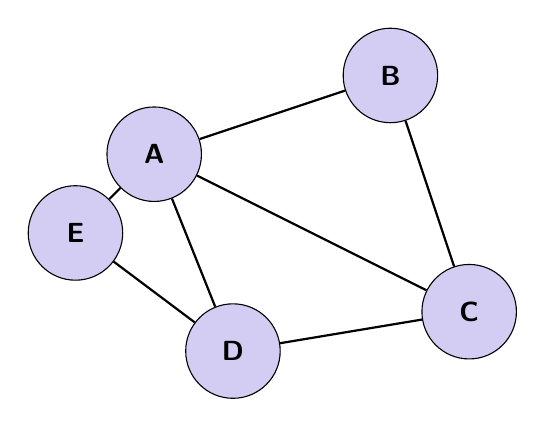
\begin{tikzpicture}[
      vertex/.style = {circle, draw, fill=blue!20,
                       minimum size=1.2cm, font=\sffamily\bfseries},
      edge/.style   = {thick}
  ]
    \node[vertex] (A) at (0,0)    {A};
    \node[vertex] (B) at (3,1)    {B};
    \node[vertex] (C) at (4,-2)   {C};
    \node[vertex] (D) at (1,-2.5) {D};
    \node[vertex] (E) at (-1,-1)  {E};

    \draw[edge] (A) -- (B);
    \draw[edge] (A) -- (C);
    \draw[edge] (A) -- (D);
    \draw[edge] (B) -- (C);
    \draw[edge] (C) -- (D);
    \draw[edge] (D) -- (E);
    \draw[edge] (E) -- (A);
  \end{tikzpicture}
  \caption{Grafo não dirigido $G_1$ com 5 vértices e 7 arestas.}
  \label{fig:grafo_nao_dirigido}
\end{figure}

Esse grafo pode modelar, por exemplo, um mapa rodoviário simplificado em que os
vértices representam cidades e as arestas representam estradas de mão dupla que
as interligam \cite{jurkiewicz2007}.

\subsection{Exemplo 2 --- Grafo Dirigido (Dígrafo)}

Considere agora o dígrafo $G_2 = (V_2,\, A_2)$ em que
\[
  V_2 = \{P,\, Q,\, R,\, S\}
  \quad \text{e} \quad
  A_2 = \{(P,Q),\, (Q,R),\, (R,S),\, (S,P),\, (P,R)\}.
\]

Nesse caso, os arcos possuem direção: por exemplo, o arco $(P, Q)$ representa
uma relação que parte de $P$ e chega em~$Q$, mas não necessariamente o
contrário. Esse tipo de estrutura é adequado para modelar, entre outros
contextos, vias de mão única em uma cidade ou o fluxo de informações em uma
rede de computadores \cite{cormen2009}.

\begin{figure}[htb]
  \centering
  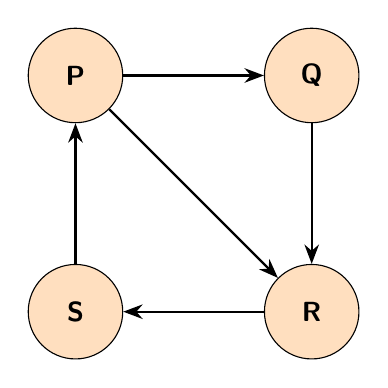
\begin{tikzpicture}[
      vertex/.style  = {circle, draw, fill=orange!25,
                        minimum size=1.2cm, font=\sffamily\bfseries},
      arc/.style     = {thick, -{Stealth[length=7pt]}},
      node distance  = 3cm
  ]
    \node[vertex] (P) at (0,0)   {P};
    \node[vertex] (Q) at (3,0)   {Q};
    \node[vertex] (R) at (3,-3)  {R};
    \node[vertex] (S) at (0,-3)  {S};

    \draw[arc] (P) -- (Q);
    \draw[arc] (Q) -- (R);
    \draw[arc] (R) -- (S);
    \draw[arc] (S) -- (P);
    \draw[arc] (P) -- (R);
  \end{tikzpicture}
  \caption{Dígrafo $G_2$ com 4 vértices e 5 arcos orientados.}
  \label{fig:digrafo}
\end{figure}

\subsection{Exemplo 3 --- Grafo Completo $K_4$}

O grafo completo $K_4$ possui $n = 4$ vértices e $\frac{4 \times 3}{2} = 6$
arestas, sendo todo par de vértices adjacente. Todos os vértices possuem grau
$\delta = n - 1 = 3$ \cite{bondy1976}.

\begin{figure}[htb]
  \centering
  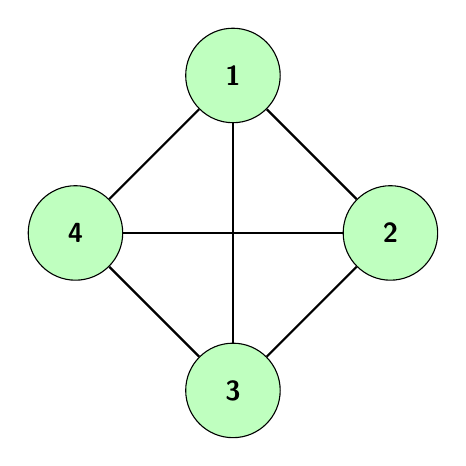
\begin{tikzpicture}[
      vertex/.style = {circle, draw, fill=green!25,
                       minimum size=1.2cm, font=\sffamily\bfseries},
      edge/.style   = {thick}
  ]
    \node[vertex] (1) at (0, 2)   {1};
    \node[vertex] (2) at (2, 0)   {2};
    \node[vertex] (3) at (0,-2)   {3};
    \node[vertex] (4) at (-2, 0)  {4};

    \draw[edge] (1) -- (2);
    \draw[edge] (1) -- (3);
    \draw[edge] (1) -- (4);
    \draw[edge] (2) -- (3);
    \draw[edge] (2) -- (4);
    \draw[edge] (3) -- (4);
  \end{tikzpicture}
  \caption{Grafo completo $K_4$ com 4 vértices e 6 arestas.}
  \label{fig:k4}
\end{figure}

Os grafos completos são frequentemente utilizados como casos-limite em problemas
de otimização combinatória, como o clássico Problema do Caixeiro Viajante, que
busca o menor caminho que passa por todos os vértices exatamente uma vez
\cite{rosen2012}.

% ----------------------------------------------------------
\section{Relação com a BNCC}
% ----------------------------------------------------------

Investigar a relevância da Teoria dos Grafos no contexto da Educação Básica e
sua relação com as competências e habilidades previstas na BNCC é essencial para
justificar sua inserção curricular. A Teoria dos Grafos é uma ferramenta
poderosa para modelar e resolver problemas do cotidiano, e sua inclusão no
currículo pode proporcionar uma abordagem mais prática e aplicada de conceitos
matemáticos, permitindo que os alunos desenvolvam habilidades críticas e
analíticas.

A Base Nacional Comum Curricular (BNCC) enfatiza a importância de desenvolver
competências que preparem os alunos para enfrentar desafios do mundo real. A
Teoria dos Grafos pode ser utilizada para:

\begin{itemize}
  \item \textbf{Desenvolvimento do pensamento computacional}: a BNCC defende a
        promoção do pensamento algorítmico e computacional, e a Teoria dos Grafos
        oferece uma linguagem matemática que pode ser utilizada para resolver
        problemas complexos, como otimização de rotas e análise de redes;
  \item \textbf{Interdisciplinaridade}: sua aplicação pode ser integrada a
        diversas disciplinas, como Ciências, Geografia e História, permitindo uma
        aprendizagem mais contextualizada e significativa.
\end{itemize}

% ==========================================================
\chapter{ESTRATÉGIAS DIDÁTICAS PARA O ENSINO DE GRAFOS}
% ==========================================================

Discutem-se, neste capítulo, potenciais estratégias didáticas para a introdução
dos conceitos de grafos no Ensino Médio, com foco em abordagens
interdisciplinares e contextualizadas.

A resolução de problemas ligados ao cotidiano é uma das maneiras de se abordar a
Teoria dos Grafos, com a recomendação de ``ênfase na resolução de problemas, na
exploração da Matemática a partir dos problemas vividos no cotidiano e
encontrados nas várias disciplinas'' \cite[p.~20]{brasil2002}.

Adicionalmente, a LDB (Lei de Diretrizes e Bases da Educação Nacional) preconiza
que as metodologias de resolução de problemas sejam adequadas ao cotidiano
discente \cite{brasil1996}. Tal diretriz busca fomentar o pensamento autônomo e a criação de
soluções próprias, permitindo que o estudante desenvolva independência na
capacidade de resolver problemas.

Assim como ocorreu em outros estados, a Bahia vem incorporando atualizações
importantes em suas diretrizes, fruto do trabalho coletivo de professores e
equipes técnicas. Entre essas iniciativas, destacam-se propostas que ampliam o
repertório matemático dos estudantes, incluindo temas que raramente aparecem no
currículo tradicional, como elementos introdutórios da Teoria dos Grafos.

Compartilhamos da ideia de \citeonline{malta2008} quando afirma que ``a Teoria
dos Grafos apresenta aspectos pertinentes que merecem espaço no currículo da
Escola Básica''. Mas, conforme apresentado no documento norteador, o que poderia
ser considerado uma introdução à Teoria dos Grafos?

Recorrendo à história, verificamos que o estudo sobre esse ramo da Matemática
surgiu com o problema das Sete Pontes de Königsberg (1736) e foi aperfeiçoado
com o \textit{Icosian Game} (1856), desenvolvidos por Leonhard Euler e William
Rowan Hamilton, respectivamente. Assim, apoiamo-nos nesse contexto histórico
para considerar que pertencem à introdução da Teoria dos Grafos aqueles conceitos
que surgiram até o século XVIII.

Como visto anteriormente, a Teoria dos Grafos foi formulada a partir de um
problema. Logo, acreditamos que a metodologia de Resolução de Problemas pode ser
utilizada para a abordagem de grafos no Ensino Médio.

Reafirmando a escolha desse caminho, as Orientações Educacionais Complementares
aos Parâmetros Curriculares Nacionais (PCN+) enfatizam que a resolução de
problemas é peça central para o ensino de Matemática, pois o pensar e o fazer se
mobilizam e se desenvolvem quando o indivíduo está engajado ativamente no
enfrentamento de desafios \cite[p.~53]{brasil2002}.

Essa competência não se desenvolve quando propomos apenas exercícios de aplicação
dos conceitos e técnicas matemáticas, pois, nesse caso, o que está em ação é uma
simples transposição analógica: o aluno busca na memória um exercício semelhante
e desenvolve passos análogos aos daquela situação, o que não garante que seja
capaz de utilizar seus conhecimentos em situações diferentes ou mais complexas
\cite[p.~112]{brasil2002}.

% ==========================================================
\chapter{CONCLUSÃO}
% ==========================================================

Contextualização inicial para apresentar o problema e ressaltar a importância do
trabalho; pequeno parágrafo para conclusão de cada título; parágrafo sobre
metodologia; um parágrafo que responde ao problema de pesquisa e, para impressionar
a banca, pode ser incluído um último parágrafo com sugestões para a continuidade
ou o aprofundamento da pesquisa.

\textit{[Nota: O autor deve desenvolver aqui o texto conclusivo definitivo
baseado nas diretrizes apontadas no seu rascunho.]}

% ----------------------------------------------------------
% ELEMENTOS PÓS-TEXTUAIS
% ----------------------------------------------------------
\postextual

\bibliography{referencias}

% ---
% Apêndices
% ---
\begin{apendicesenv}
\partapendices

\chapter{Subtítulo do apêndice}
Apêndices têm o objetivo de melhorar a compreensão textual, ou seja, completar
ideias desenvolvidas no decorrer do trabalho.

\end{apendicesenv}

% ---
% Anexos
% ---
\begin{anexosenv}
\partanexos

\chapter{Subtítulo do anexo}
Anexos são elementos que dão suporte ao texto, mas que não foram elaborados pelo
autor.

\end{anexosenv}

\end{document}